\section{Working Principle}

Every type of wireless data transmission only transmits in a designated frequency. It would get crowded in the air when many users 
are on a single channel. Think about traffic on the highway, there should be multiple lanes designated for different purposes. 
All the vehicles drive on their lane based on the rule. You have roadways, passing lanes, carpool lanes, emergency lanes, etc. 
It will get very crowded on the roadways during certain times of the day due to high volume of cars, where less or no one is 
using any of the carpool lanes or emergency lanes. This occurs in wireless communication, too. Different channels or frequencies
are assigned to different public organizations, private sectors or other stations. 
During certain times of the day, people use their typical devices, which may transmit data only on a designated channel.
This is the same situation as traffic is all crowded in one lane. Integrating a cognitive radio network is basically adding a traffic light or employing highway patrol for the busy channels. When primary users are not using their license band, they are considered open channels. If the no one do anything to it, this results in very low utilization. The main idea for Cognitive Radio Network is to create
a smart networking environment for a secondary user (SU) to use those idle bands. SU is free to use the band as long as the 
primary user (PU) is not here. When the PU of the band comes, SU must handoff to another band that is free. Generally, using
such handoff mechanism, it increases the spectrum utilization overall. 


\section{Application}

One utilization of the cross channels transmission mechanism enables a way to implement Internet of Things (IoT), which means
everything in life can share their obtained knowledge with everything else. 
IoT helps automated machines to make better 
decisions in real time. IEEE standard 802.22.3, or now transiting to 802.15, has designated working groups in IoT area
\cite{ieee_working_group}. Electric devices like smart refrigerator, smart fan, or smart lamp is mostly connected online
using WiFi or Zigbee technology. The transmission load will eventually overwhelm both spectrum ranges as the devices scale
up. With cognitive radio technology, it will help release some of the stress from these bands.

Because of the nature of the radio frequency that CR uses, it also can be applied very well at sub-urban areas and big cities.
In theory, it can transmit as far as 100 kilo-meter range as Figure~\ref{fig:radio_range} demonstrates. These numerical values are obtained from IEEE standards and their specification. The only drawback
is, even as the signal is traveling at the speed of light, it inevitably has minor delay for every transmission. For those
applications that put latency metric as least priority, that wouldn't be an issue. It can still work well with essential
rural communication, traffic division, emergency broadcast, etc. 


\begin{figure}[ht]
\centering
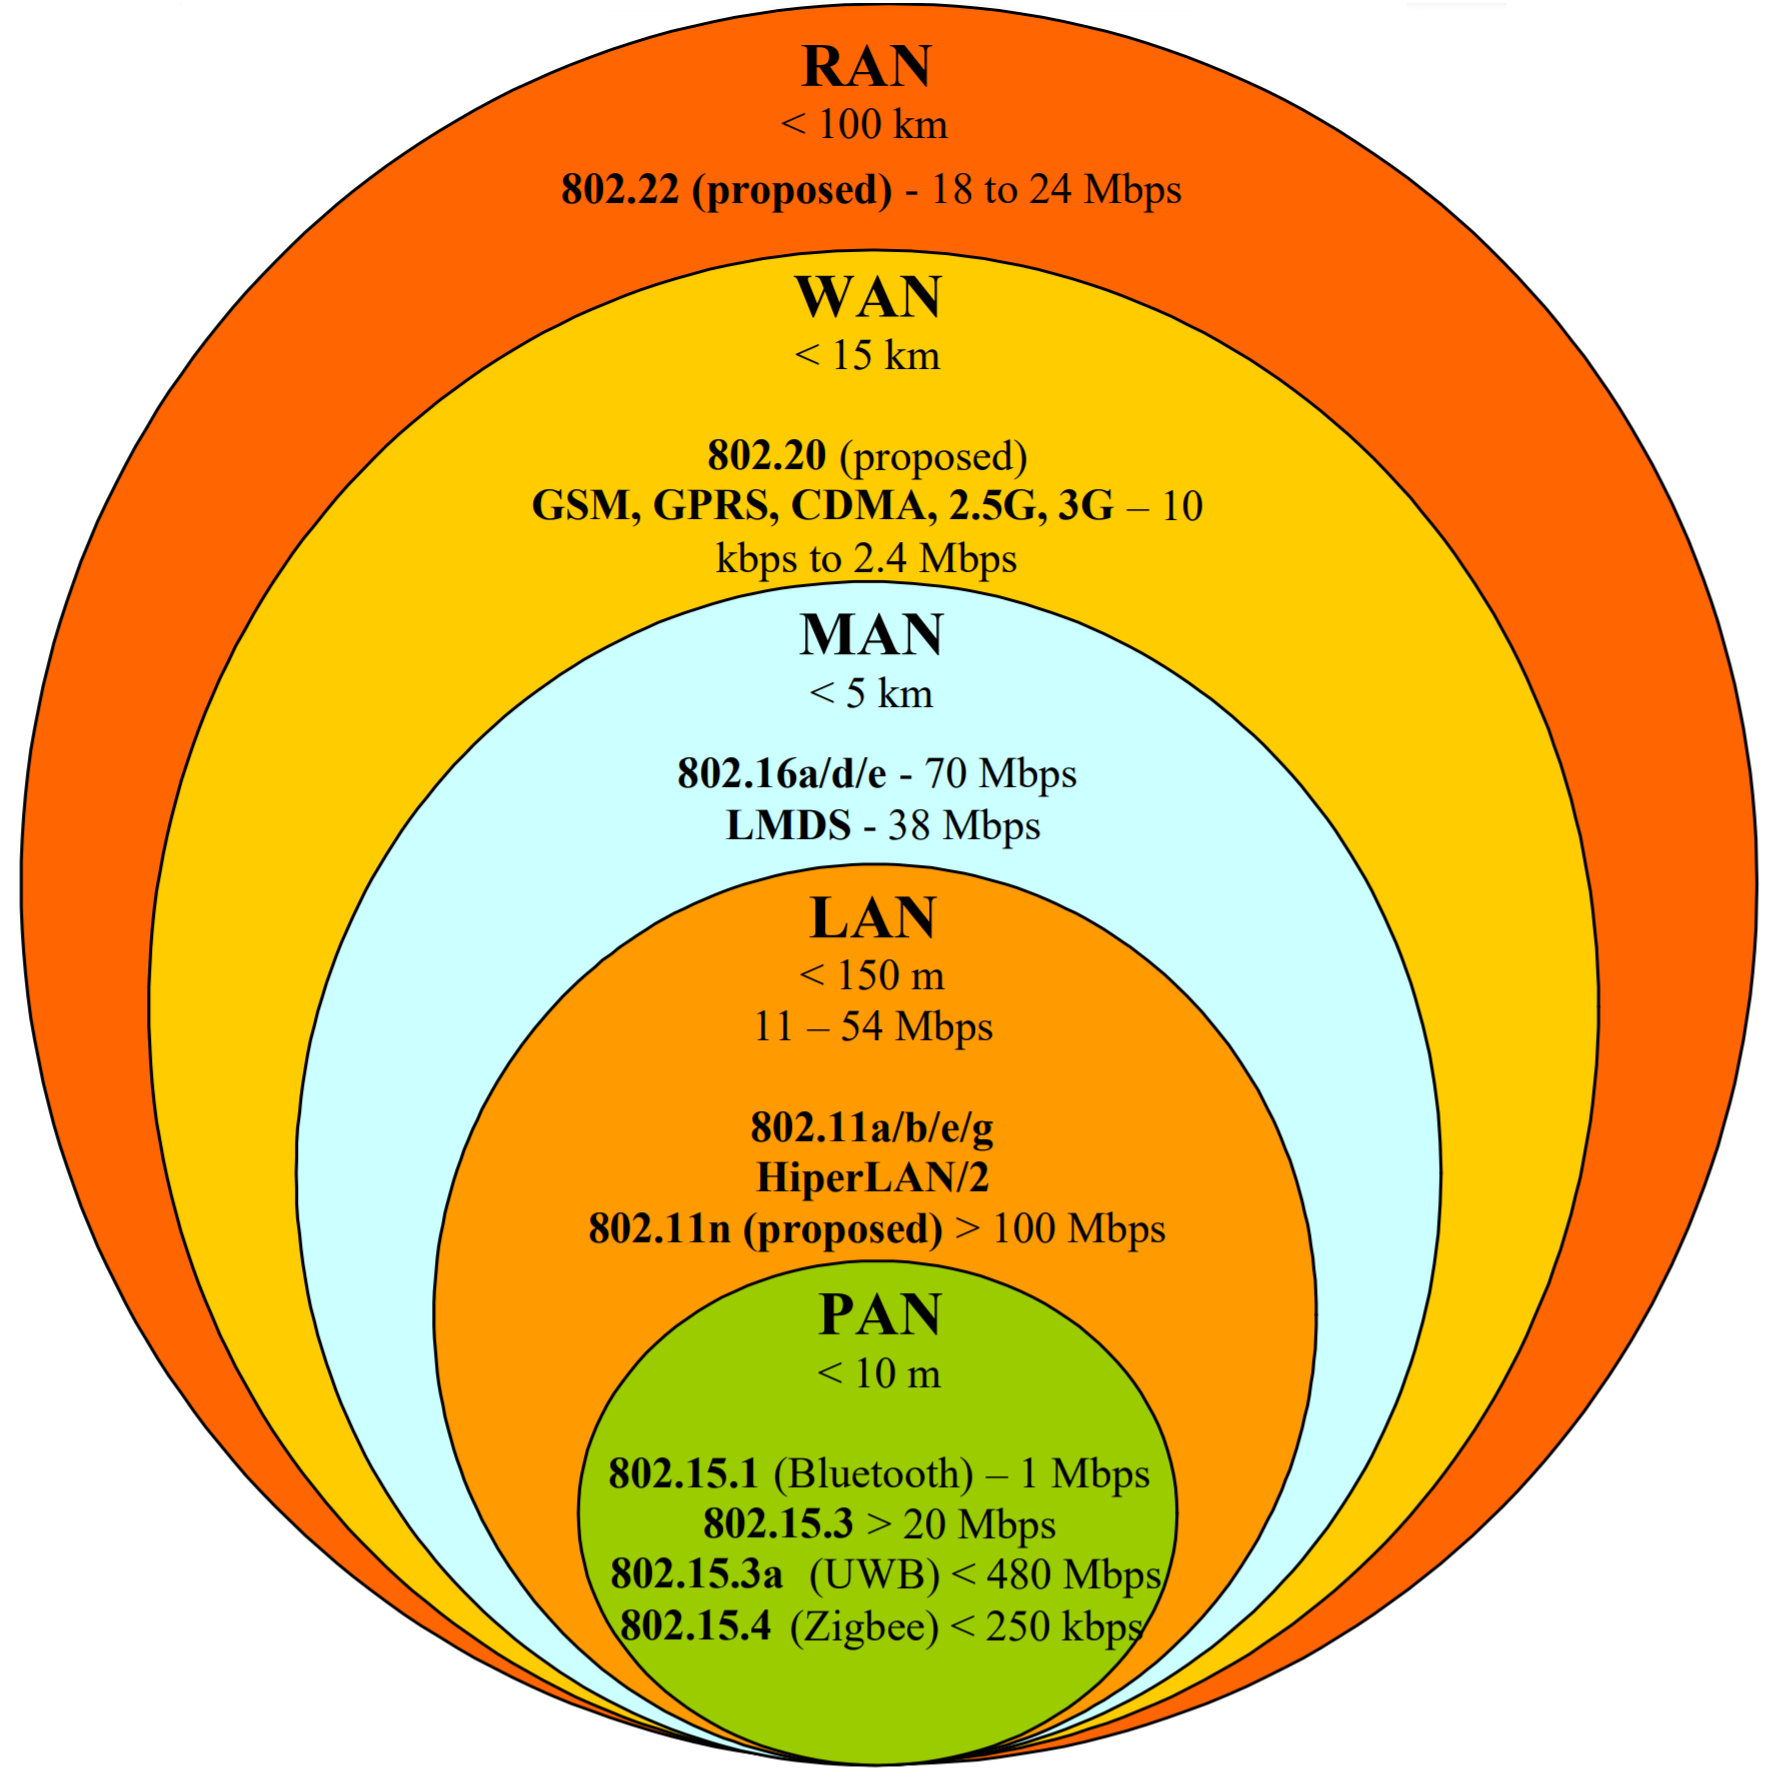
\includegraphics[width=10cm]{figures/radio_range.png}
\caption{Radio Standard Range \cite{ieee_802_22}}
\label{fig:radio_range}
\end{figure}

Continuing the topic of CRN limitation, disturbance is another concern for the licensed band users. Due to imperfection of
the CR system, during PU operation hours, if another SU is also transmitting, it would be considered as noise to the 
primary services. PU would like to discourage such technology if any of these interruptions happen frequently. However, during non-operation hours, the band owners could sub-lease their bands to anyone who uses CR. This potentially bring a
market and demand of the shareable network.

\section{History}
After discussing so much of the application opportunity of the CRN, let's revisit the history of the technology with 
more appreciation. The idea of cognitive radio was first introduced by Joseph Mitola III at KTH in 1998. It sounded 
merely just another idea to organize the band usage. People knew this is a way to maximize band utilization after all.
Not long after that, in the year 2000, there was a huge explosion in a Netherlands firework factory \cite{cr_history}. 
23 people were killed. Local emergency hotlines faced serious communication issue during the crisis which lead to further
deterioration and destruction. This same problem happened during 9/11 in the United States in 2001. These incidents
pushed intellectual and academic societies to work towards developing a better management system for the electromagnetic
spectrum. People realize CR is not just a tool help setting up extra communication channel when under load, it
potentially open up emergency lines to save lives. With higher precaution awareness and a rising demand on data usage, such as IoT applications, in our time, managing the frequencies properly is the top priority. With the goals and current technology, scientists and engineers
begin to work on different areas relating to optimizing and setting up the network.

The first cognitive radio standard IEEE 802.22 was published by IEEE 802 LAN/MAN Standard Committee (LMSC)in 2011. 
IEEE 802 Part 22 also known as Wireless Regional Area Networks (WRAN) standard. It specified geolocation and spectrum
sensing methodology. Geolocation relies on a databases composed of licensed transmitters in the area and geographical 
realm for the CRN. For a CR device, each is capable of sensing the channel status (busy or idle). It also needs to be 
capable of sensing the source of the frequency in the air. Spectrum sensing often utilize one of the following, energy 
detector, matched filter, cyclostationary process. Energy detection is by far the most used way in radio-frequency 
integrated circuit (RFIC) chips. 


\section{Characteristics}
IEEE 802 Part 22 states an entire regulation on the policies and procedures for operating in the TV bands. 
Table~\ref{tab:physical} summarize the key points in the Physical Layer (PHY) specifications. For TV bands, 
the transmit frequency in the air generally set between at the very high frequency (VHF) and the ultra high frequency (UHF) range
for quality and long distance data transmission. Depends on the regions, channel bandwidth can be varied which lead to
different throughput values. The overall throughput of the data flow can go up to 22.69 Mbit per second.
The modulation method can adapt to the most usable technology at the current time and space. 


\begin{table}[ht]
\centering
\setlength{\tabcolsep}{20pt}
\renewcommand{\arraystretch}{1.5}
\begin{tabular}{| l | l |}
\hline
\hspace{0.3cm}  Environment & TV broadcast white space \\ 
\hline
\hspace{0.3cm}  Frequency range &  54 - 862 MHz  (VHF - UHF)\\ 
\hline
\hspace{0.3cm}  Channel bandwidth &  6, 7 or 8 MHz \\ 
\hline
\hspace{0.3cm}  Throughput &  4.54 - 22.69 Mbs  \\ 
\hline
\hspace{0.3cm}  Modulation &  QPSK, 16-QAM or 64-QAM  \\ \hline
\hline
\end{tabular}
\caption{Physical Layer Characteristics}
\label{tab:physical}
\end{table}

Moving on to the Cognitive WRAN Medium Access Control (MAC) specifications. As states in IEEE 802.22, devices should have 48
bits MAC address for identification in the net. Connections between devices should also have 12 bits Company Identifier (CID). The 
connections are assembled with a stream of data, called superframe. A superframe is constructed of a preamble, synchronize channel (SCH) and 16 frames
in total. Figure~\ref{fig:frame} shows the transmission through a time period and the frame structure at a couple of the opened channels in the TV band. The red bars across time indicate there are occupations to the TV channels at the specific frequencies. Yet, the system shown should spot the idle channels in the middle at around some frequency of t. And it begins the channel synchronization process by sending preamble and SCH to the channel. After it is in sync, secondary devices can exchange data in the frames. 

\begin{figure}[ht]
\centering
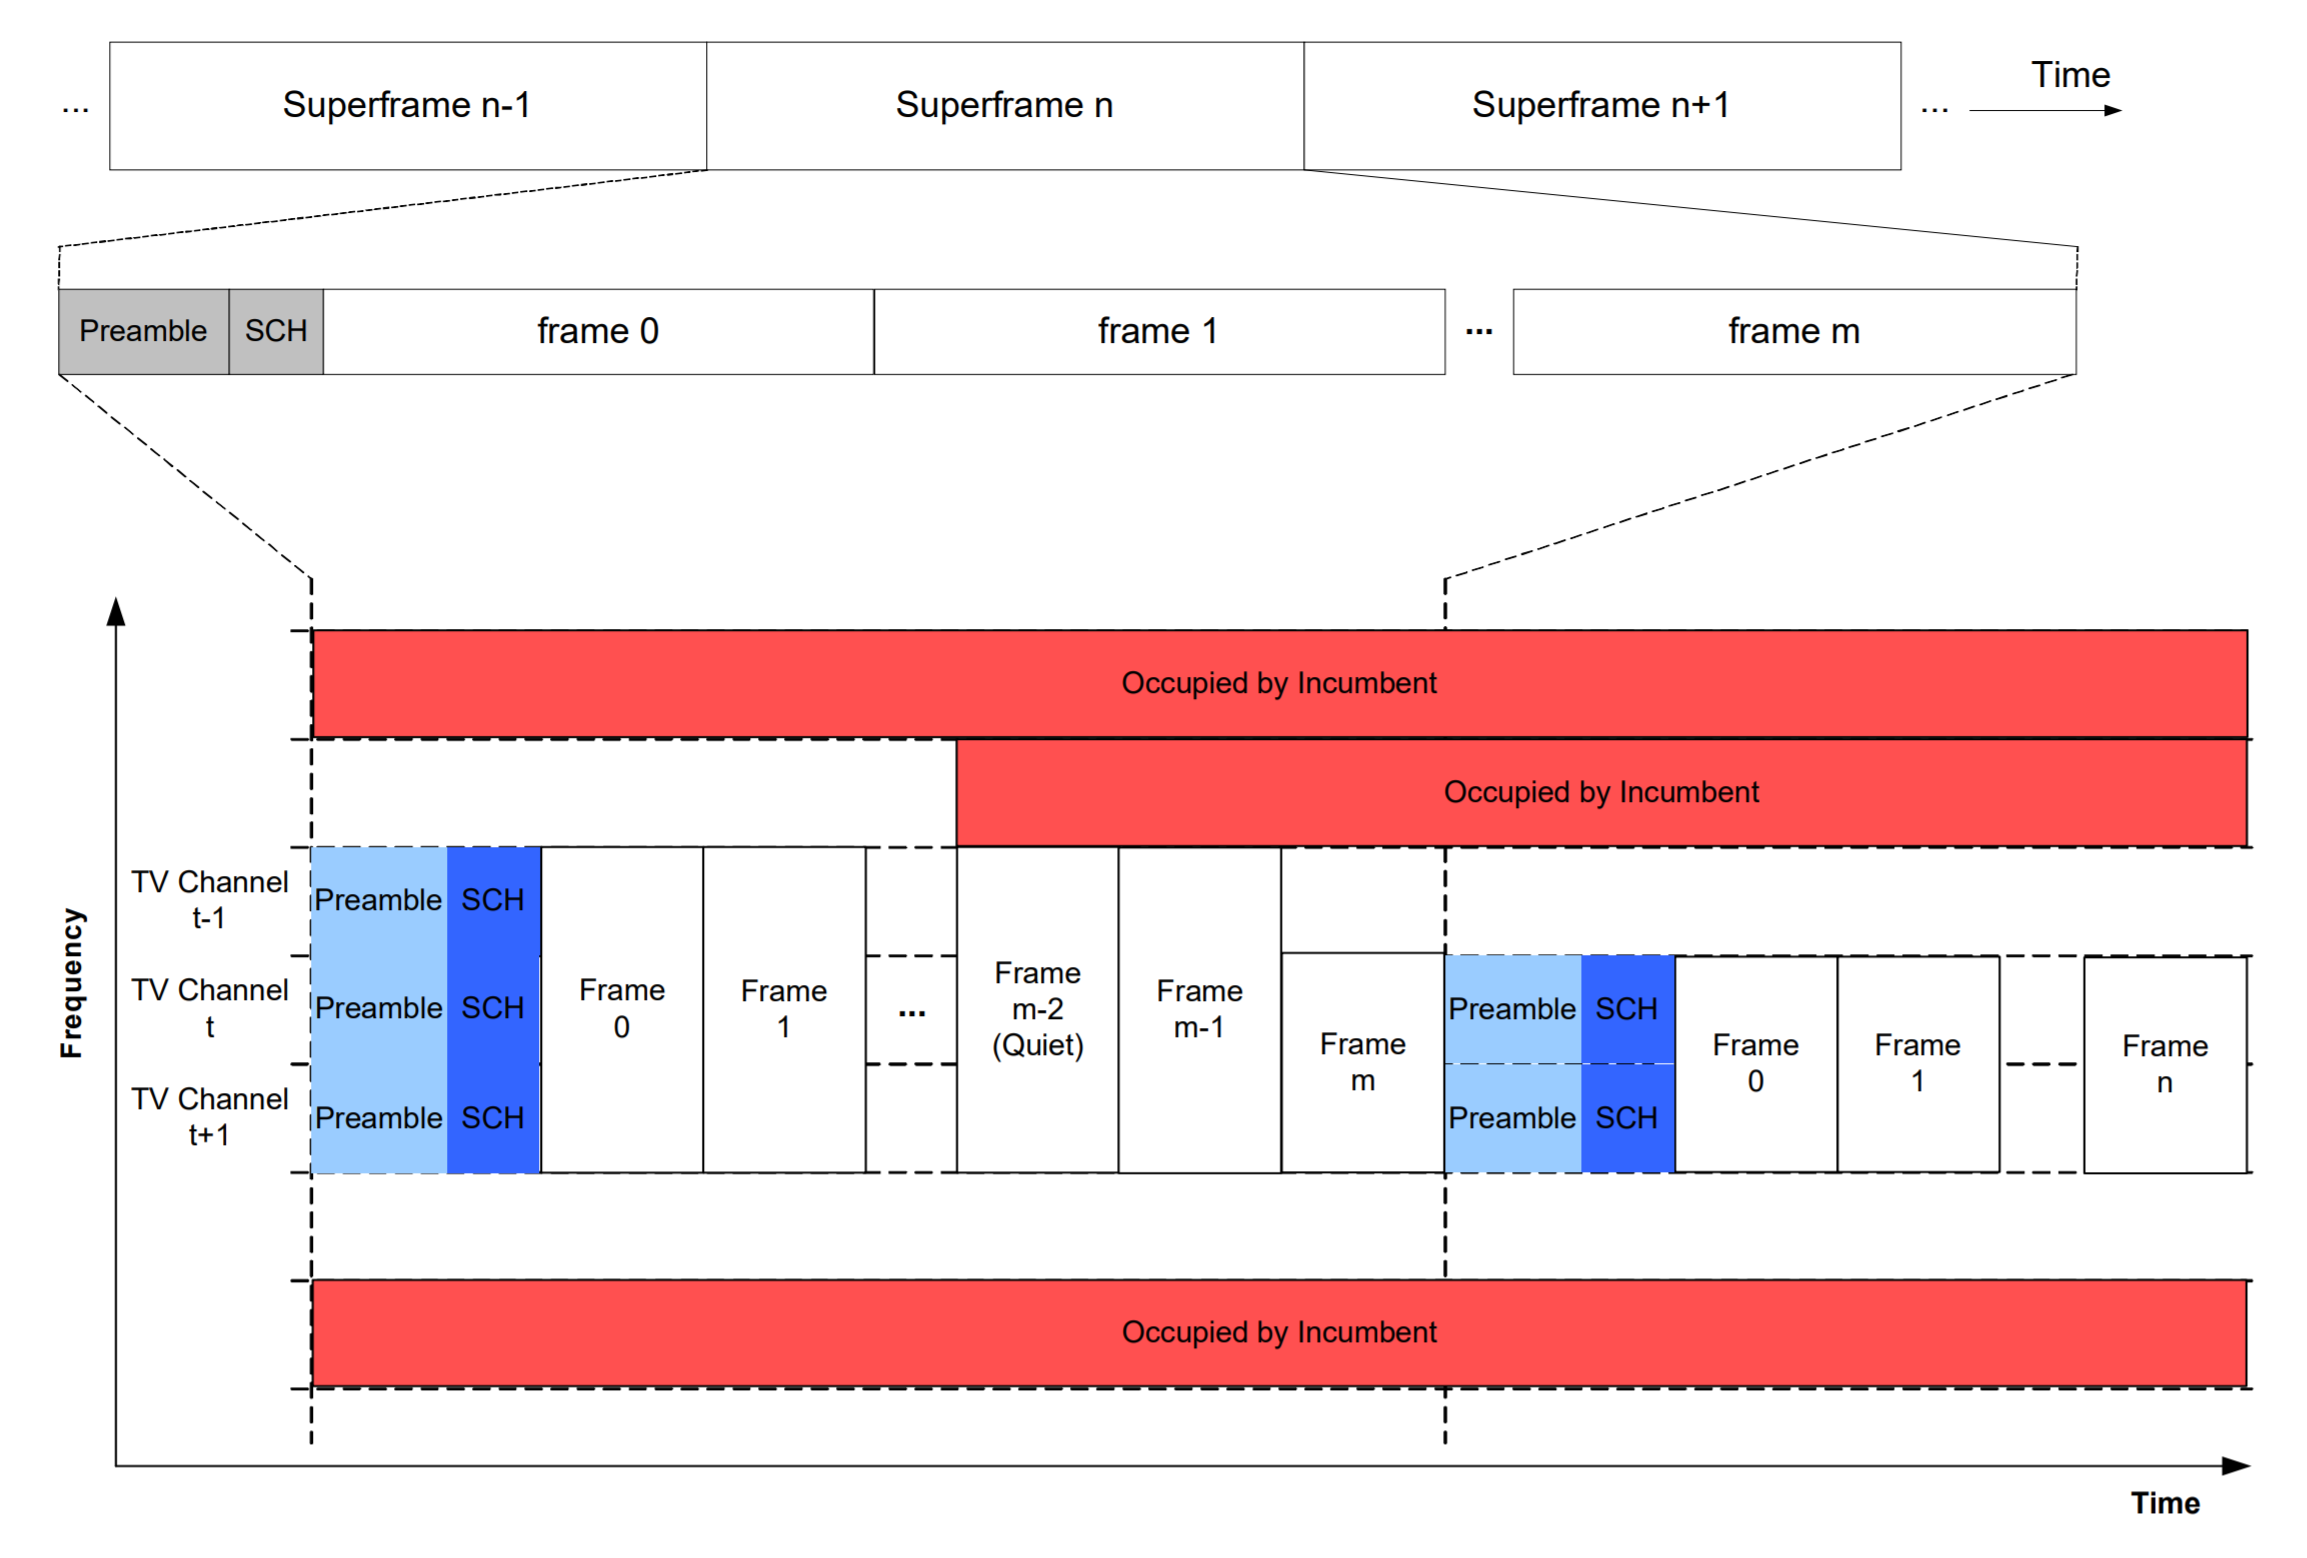
\includegraphics[width=12cm]{figures/frame.png}
\caption{Frame Structure \cite{ieee_802_22}}
\label{fig:frame}
\end{figure}

When implementing CR device, regulation suggests to take note of the following hardware characteristics:
\begin{itemize}
  \item Receiver sensor sensitivity 
  \item Channel sensing time
  \item Hit rate
  \item False alarm
\end{itemize}
Looking at the sensitivity of the device, a better sensor senses and reacts to the environment in much longer range and shorter 
time. Hit rate and false alarm of the hardware relate closely to the system integration design. You can find most of these statistical
value in the datasheet of the module parts.

